\documentclass[a4paper.12pt]{article}
\usepackage[top=2cm, bottom=2cm, left=2.5cm, right=2.5cm]{geometry}
\usepackage[brazil]{babel}
\usepackage[utf8]{inputenc}
\usepackage[T1]{fontenc}
\usepackage{amsmath, amsfonts, amssymb}
\usepackage{indentfirst}
\usepackage{graphicx}
\usepackage{hyperref}
\usepackage{float}
\usepackage{cite}
\title{problema dos três corpos}
\author{Allison Eduardo de Sousa Bonfim\\ mackhyuuga@hotmail.com}
\date{20/02/2020}

\begin{document}

\maketitle
\newpage

\tableofcontents

\section{descrição do código}

\subsection{resumo}

O problema de três corpos trata de objetos puntiformes, dimensões desprezíveis, interagindo mutuamente através da força gravitacional de Newton. Ao longo de mais de três séculos, o estudo deste tipo de sistema levou ao desenvolvimento e ao aprimoramento de diversas técnicas matemáticas, tanto analíticas quanto numéricas, para a compreensão de problemas que envolvem sistemas dinâmicos. Este trabalho tem como objetivo desenvolver e discutir alguns desses resultados aplicados ao problema de três corpos restrito, formulado a partir da segunda lei de Newton.


\subsection{descrição do problema físico}

	O problema consiste em descrever o movimento de três partículas que interagem por força gravitacional. Sejam três massas $m_1$, $m_2$ e $m_3$ no $\mathbb{R}^3$ indexadas pelos vetores $\vec{r_1}$, $\vec{r_2}$, $\vec{r_3}$. Pelas leis de Newton e pelo princípio da superposição, podemos chegar nas seguintes equações diferenciais de segunda ordem.
	
	\begin{equation}
	m_1\dfrac{d^2\vec{r_1}}{dt^2}=\dfrac{Gm_1m_2}{|\vec{r_{12}}|^3}(\vec{r_2}-\vec{r_1})+\dfrac{Gm_1m_3}{|\vec{r_{13}}|^3}(\vec{r_3}-\vec{r_1})
	\end{equation}
	\begin{equation}
	m_2\dfrac{d^2\vec{r_2}}{dt^2}=\dfrac{Gm_2m_3}{|\vec{r_{23}}|^3}(\vec{r_3}-\vec{r_2})+\dfrac{Gm_2m_1}{|\vec{r_{21}}|^3}(\vec{r_1}-\vec{r_2})
	\end{equation}
	\begin{equation}
	m_3\dfrac{d^2\vec{r_3}}{dt^2}=\dfrac{Gm_3m_2}{|\vec{r_{32}}|^3}(\vec{r_2}-\vec{r_3})+\dfrac{Gm_3m_1}{|\vec{r_{31}}|^3}(\vec{r_1}-\vec{r_3})
	\end{equation}
	Sendo $G$ a constante da gravitação universal, ao longo desse trabalho assumirei que $G=1\dfrac{Nm^2}{kg^2}$, e $\vec{r_{ij}} = \vec{r_i} - \vec{r_j}$. Ao invés de se trabalhar com essas três equações diferenciais de segunda ordem, pode-se fazer $\vec{v_i}=\dfrac{d\vec{r_i}}{dt}$ e conseguentimente $\dfrac{d\vec{v_i}}{dt}=\dfrac{d^2\vec{r_i}}{dt^2}$. Obtendo, assim, seis equações vetoriais diferenciais de
	primeira ordem ou doze equações escalares. As equações referentes a $m_1$ se encontram abaixo:  
    
    \begin{equation}
		\begin{cases} \label{gravity}
			\dfrac{dv_{1x}}{dt}=\dfrac{m_2}{|\vec{r_{12}}|^3}(x_2-x_1)+\dfrac{m_3}{|\vec{r_{13}}|^3}(x_3-x_1)
			\\
			\dfrac{dr_{1x}}{dt}=v_{1x}
			\\\\
			\dfrac{dv_{1y}}{dt}=\dfrac{m_2}{|\vec{r_{12}}|^3}(y_2-y_1)+\dfrac{m_3}{|\vec{r_{13}}|^3}(y_3-y_1)
			\\
			\dfrac{dr_{1y}}{dt}=v_{1y}
		\\\\\end{cases} 
	\end{equation}
	
	As definições apresentadas também podem ser usadas, com algumas mudanças, para corpos cujas dimensões não sejam desprezível. Para o caso de um distribuição esfericamente simétrica, pode-se aplicar as equações apresentadas supondo que toda a massa está concentrada em seu centro. Esse resultado foi obtido por newton em 1685 e sua demonstração pode ser encontrada em \cite{Nussenzveig}.

\subsection{métodos e análise numérica}
Foi provado por poincaré em 1980 que este problema é insolúvel por quadratura, assim sendo, são somente possíveis séries de aproximações e não uma solução analítica para o mesmo. O método numérico escolhido para resolver as equações diferenciais foi o runge kutta 4 ordem.

A minha intenção inicial é fazer um programa que, a partir das condições iniciais, calcule a força na particula $1$ devido a $2$ e $3$, assim descobrindo a sua aceleração e a sua trajetória durante um intervalo pequeno de tempo, o mesmo será feito para $2$ e $3$. Então, tendo a posição de $\vec{r_{1}}(t+dt)$, $\vec{r_{2}}(t+dt)$, $\vec{r_{3}}(t+dt)$; o procedimento se repetirá. O objetivo é que após $n$ interações tenhamos a descrição da orbital em um intervalo de tempo significativo.

\subsection{runge kutta de quarta ordem}
Seja um sistema de equações diferenciais com valor inicial \\\\
\begin{equation} \label{equação}
	\begin{cases}
		y_1'=f_1(x,\,y1\,,y2\,,...,\,yn), \;\;\;\;\;\;\;\;\;\; y_1(x_0) = y_{1,0} \\
		y_2'=f_2(x,\,y1\,,y2\,,...,\,yn), \;\;\;\;\;\;\;\;\;\; y_2(x_0) = y_{2,0}\\
		\vdots\\
		y_n'=f_n(x,\,y1\,,y2\,,...,\,yn), \;\;\;\;\;\;\;\;\;\; y_n(x_0) = y_{n,0}
	\end{cases}\\
\end{equation}

$\\$
podemos encontrar uma aproximação numérica para o mesmo atráves de

\begin{equation}
	\textbf{y}_{n+1}=\textbf{y}_n + \dfrac{h}{6}(\textbf{k}_1+2\textbf{k}_2+2\textbf{k}_3+\textbf{k}_4) 
\end{equation}


 $$\\\textbf{k}_1=\textbf{f}(x_n,\textbf{y}_n)$$
 $$\\\\\textbf{k}_2=\textbf{f}(x_n+\dfrac{h}{2},\textbf{y}_n+\textbf{k}_1\dfrac{h}{2})$$
 $$\\\\\textbf{k}_3=\textbf{f}(x_n+\dfrac{h}{2},\textbf{y}_n+\textbf{k}_2\dfrac{h}{2})$$
 $$\\\\\textbf{k}_4=\textbf{f}(x_n+h,\textbf{y}_n+\textbf{k}_3h)$$
		
\subsection{explicação do código}


	O código é composto por três partes. A parte da resolução númerica, feita em fortran 95, tem como objetivo pegar as condições inciais de um arquivo "entrada.txt" $\,$ calcular as orbitas dos objetos e escrever os resultados em "resultados.txt". O segundo programa, este em python, tem como função usar os dados gerados pelo programa em fortran para produzir os gráficos. Já o terceiro feito em JavaScript foi usado para produzir algumas animações referentes ao movimento dos objetos.
	
	O meu objetivo enquanto escrevia o código era mantê-lo o mais genérico possível, assim caso queira usá-lo para resolver um outro sistema de equações diferenciais, o número de mudanças a serem feitas serão mínimas. Essas alterações consistem basicamente em mudar as funções existentes em subroutine. 
	

\section{resultados e análise de dados}
\subsection{resultados}

	\begin{figure}[H]
		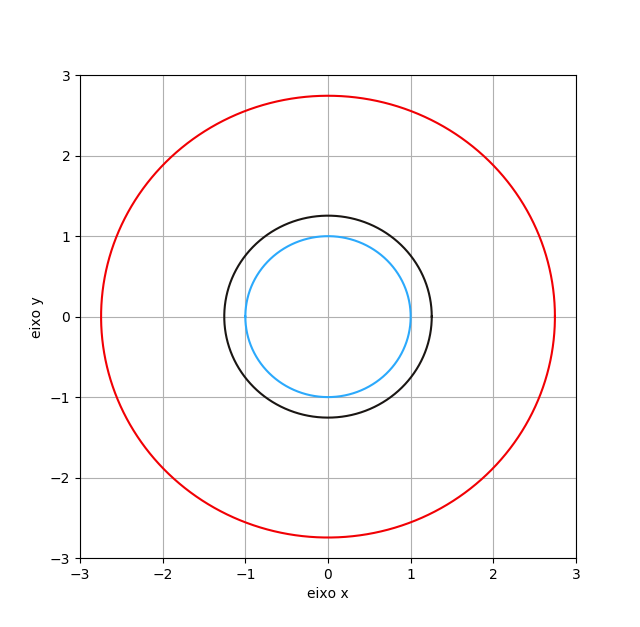
\includegraphics[scale=0.5]{Figure_1.png}
		\label{figura_1}
		\caption{\url{https://editor.p5js.org/mackhyuuga/present/bJTuIIqZ}}
		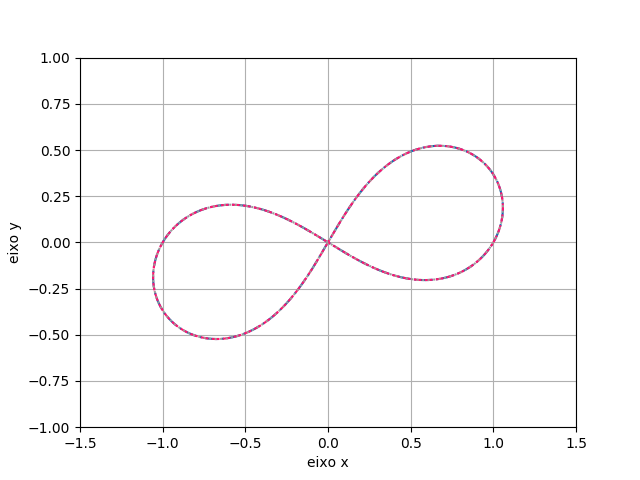
\includegraphics[scale=0.5]{Figure_2.png}
		\caption{\url{https://editor.p5js.org/mackhyuuga/present/9P_W_EO9}}
	\end{figure}
	
	A primeira imagem é a solução do problema de três corpos obtida em 1763, por Leonhard Euler \cite{euler1767motu}. A outra é a solução em oito, obtida numericamente com o auxílio computacional por Cristopher Moore, em 1993 \cite{moore}, e comprovada pouco tempo depois pelos matemáticos Alain Chenciner e Richard Montgomery \cite{chenciner2000mathematics}.
	
	A seguir algumas orbitas cujas condições iniciais foram obtidas em \cite{orbitas}.
	
	\begin{figure}[H]
		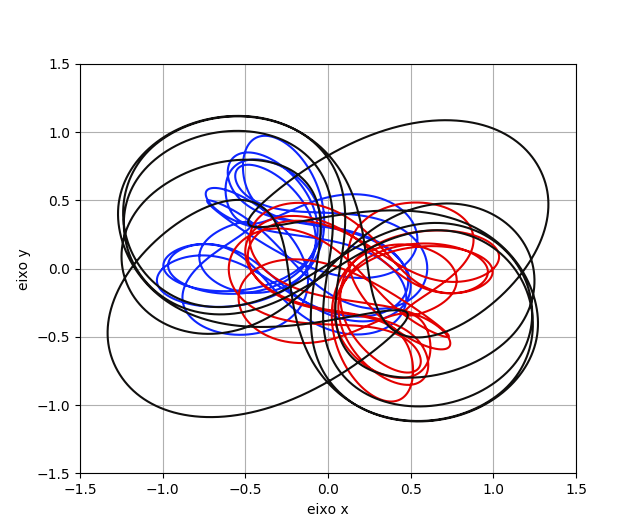
\includegraphics[scale=0.5]{Figure_8.png}
		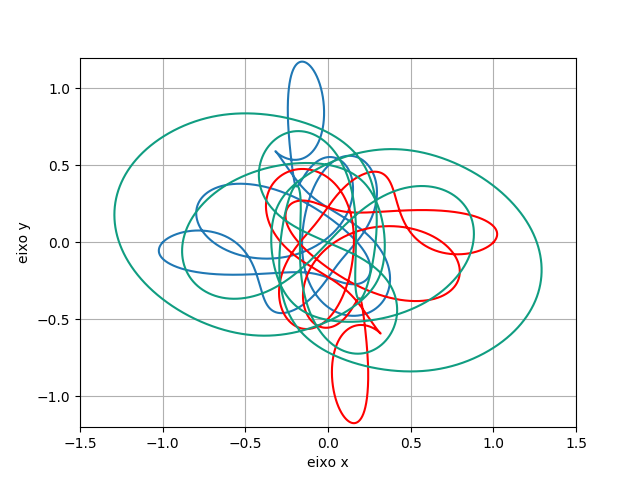
\includegraphics[scale=0.5]{Figure_13.png}
		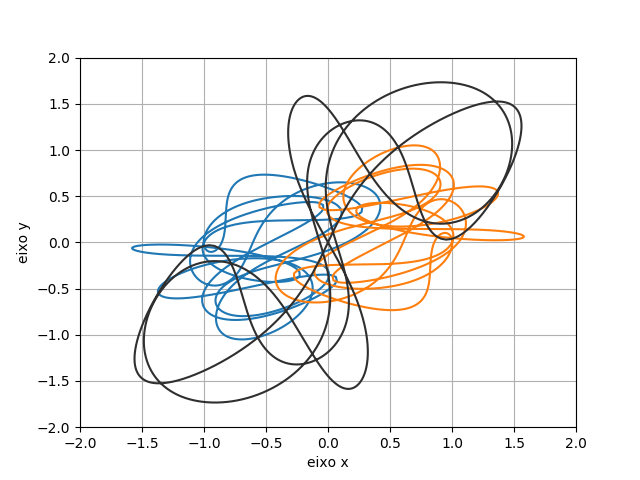
\includegraphics[scale=0.5]{Figure_14.png}
		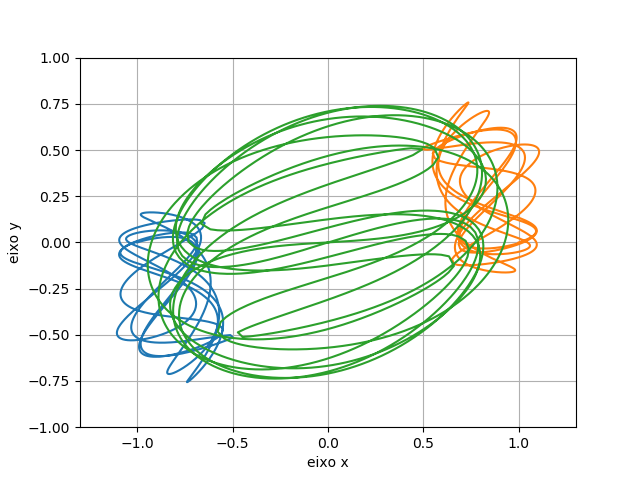
\includegraphics[scale=0.5]{Figure_7.png}
		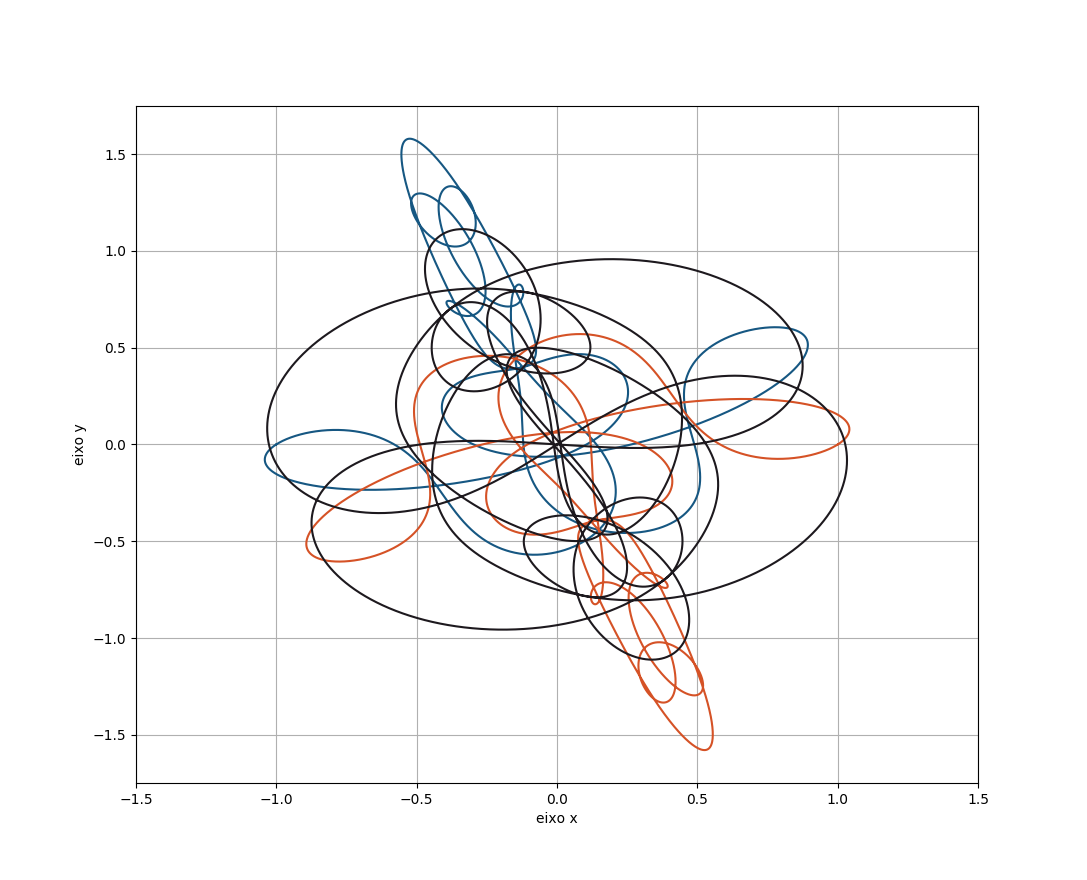
\includegraphics[scale=0.3]{Figure_12.png}
		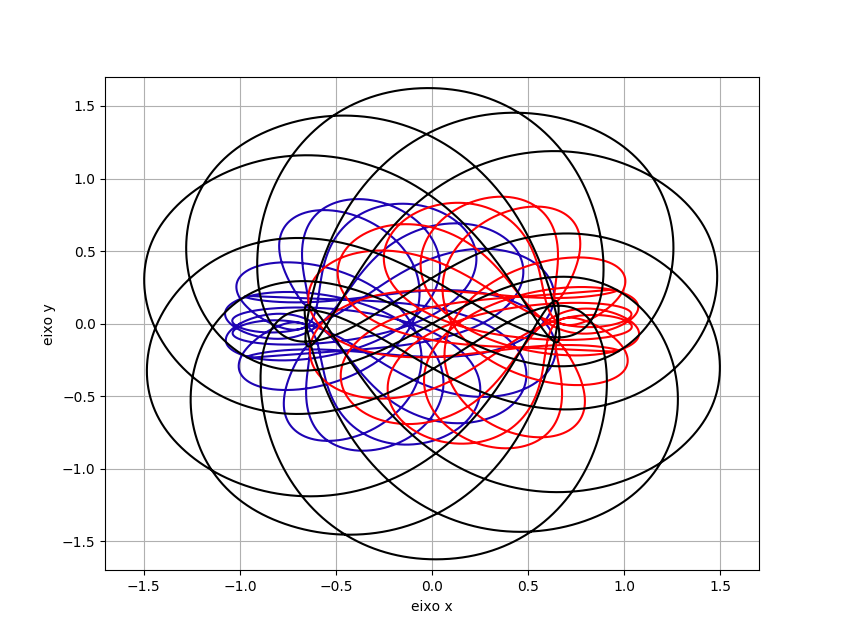
\includegraphics[scale=0.4]{Figure_9.png}
	\end{figure}
	\begin{figure}[H]
		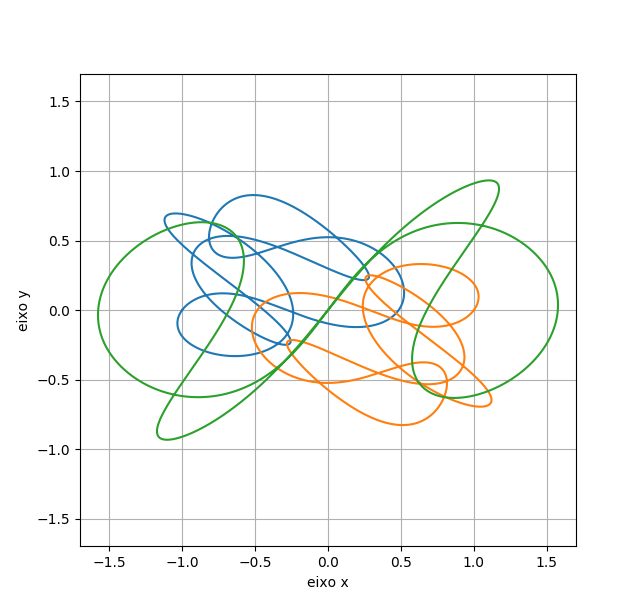
\includegraphics[scale=0.5]{Figure_11.png}
		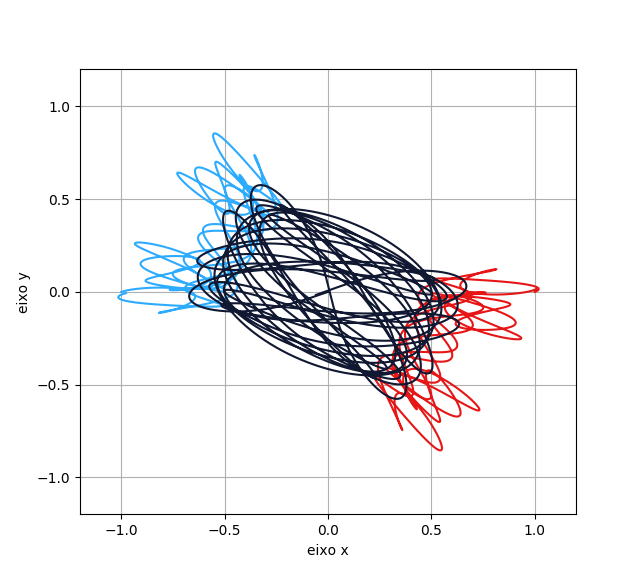
\includegraphics[scale=0.5]{Figure_10.png}
		\caption{\url{https://editor.p5js.org/mackhyuuga/present/mmKXya9x}}
		\caption{\url{https://editor.p5js.org/mackhyuuga/present/l_DgLy_i
		}}
		\caption{\url{https://editor.p5js.org/mackhyuuga/present/NlpjJj_x}}
		\caption{\url{https://editor.p5js.org/mackhyuuga/present/pz5hbB9v}}
		\caption{\url{https://editor.p5js.org/mackhyuuga/present/WXWM16ow}}
		\caption{\url{https://editor.p5js.org/mackhyuuga/present/vXuAw84s}}
		\caption{\url{https://editor.p5js.org/mackhyuuga/present/j91lxyaY}}
		\caption{\url{https://editor.p5js.org/mackhyuuga/present/A8qEBvkt}}
	\end{figure}	
	
	Segue o código que gerou as animações: \url{https://editor.p5js.org/mackhyuuga/sketches/cpap5p2Z}
	
	
	\clearpage
\subsection{análise de dados}

	Os resultados foram bastante satisfatórios, no caso das três orbitas concêntricas \ref{figura_1} por exemplo foi facil analisar a incerteza das posições uma vez que os raios dos circulos deveriam se manter constante e de fato se mentiveram com um erro relativo máximo de 2\% ao longo de 17.1655 segundo, tempo necessário para que o objeto completasse uma volta. Esse erro pode ser explicado com base nas condições iniciais pois o sistema é bastante sensível à esses valores e sua precisão, esses detalhes são discutidos em maior profundidade no artigo que estou usando como base \cite{coreografias}. Para finalizar deixo essa que foi a imagem mais bela que consegui produzir com o sistema de três corpos.
	
	\begin{figure}[H]
		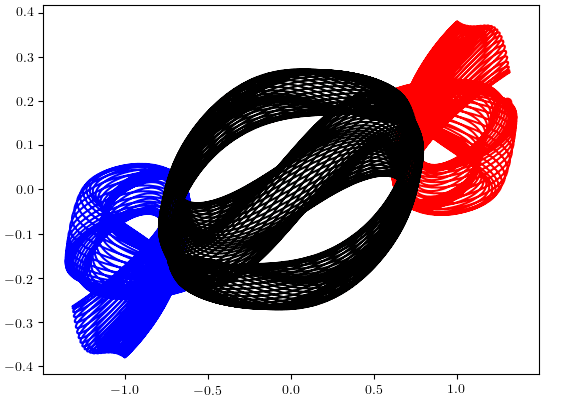
\includegraphics[scale=0.75]{Figure_3.png}
	\end{figure}
	
\clearpage
\bibliographystyle{plain}
\bibliography{referencia}
\addcontentsline{toc}{section}{referência}

\end{document}